%! suppress = MissingImport
\chapter{Introduction}
\label{cha:introduction}

%\todo[inline]{Electric vehicles are the future}
On today's day and age, the global concern on climate
change has been a major focus on recent international agreements,
such as the Paris Agreement \citep{parisAgreement},
incentivating many car manufacturers to introduce
\gls{EVs} as the eco-friendly
solution for sustainable transport for the future.

%\todo[inline]{EV autonomy}

As \gls{EVs} have been increasing in popularity in
recent years \todo{citar}, car manufacturers have
increased competitiveness on vehicle's performance,
a decisive factor for consumers \citep{EGBUE2012717}.

%\todo[inline]{ERange estimation}

A vehicle's autonomy alson knwon as \gls{eRange},
can be estimated through many driving data parameters,
such as vehicle design, driver's behavior, wheather,
road inclination and gls{SOC} estimation.
The \gls{eRange} accuracy allows consumers to rely
on its vehicle for longer travel time and efficient
charging plans \todo{citar}, \gls{eRange} estimation
however, is a complex problem whitch has prompted
previous studies in the past to provide a solution 
\citep{classicEVX, predictionOfeRange}.

%\todo[inline]{TODO: Mensionar IA na atualidade}
Machine learning is offen a viable tool for complex
problem-solving \todo{citar}, due to its nature
of quickly finding suboptimal solutions,
closest the best case scenerio possible.
The \gls{eRange} estimation problem could be solved
with \gls{machineLearning}, requiring an initial
phase to learn from the model and estimating
through realtime \gls{SOC} variations.
This project approaches the \gls{eRange} estimation
problem with the use of \gls{machineLearning} based
model to increase its accuracy.

%\todo[inline]{Prior work}
Prior work \citep{classicEVX} on \gls{eRange}
estimation demonstrated that using an
history-based algorithm on am adaptive model
provides a more reliable \gls{eRange} prediction
than a basic \gls{SOC} - manufacturer data relation,
this is mainly due to taking into account the
vehicle's driving history.
%\todo[inline]{What will be done}

The model receives a \gls{dataset} containing multiple
trips and their respective vehicle power consumption [kW]
and the vehicle speed [km/h] in a  time series format.
\todo{explicar time series format}
After training the model with the dataset,
\gls{eRange} prediction is possible through
\gls{SOC} monitoring based on previous \gls{dataset} values.
The following figure represents an overview of the system:

%! suppress = MissingLabel
\begin{figure}[H]
    \begin{center}
        %! suppress = MissingLabel
        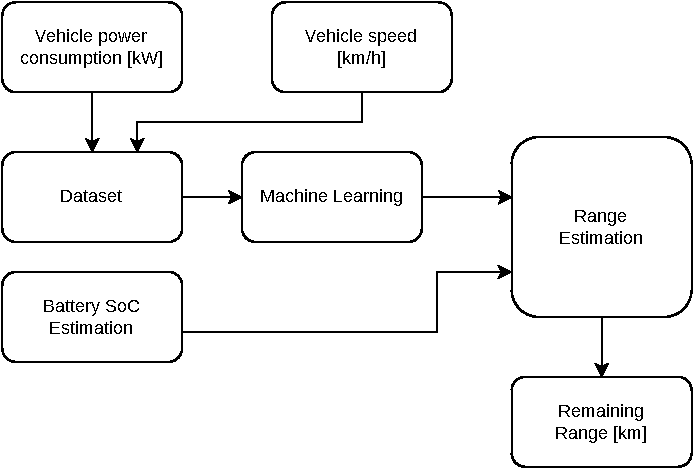
\includegraphics[scale=1.0]{../figures/generic_diagram}
        \caption{System overview.}
    \end{center}
\end{figure}

\todo[inline]{detail}